\section{Немного о курсе}

\begin{frame}{Преподаватели}
\begin{multicols}{2}

Георгий Калашнов \\
go9513@gmail.com
\begin{figure}
    \centering
    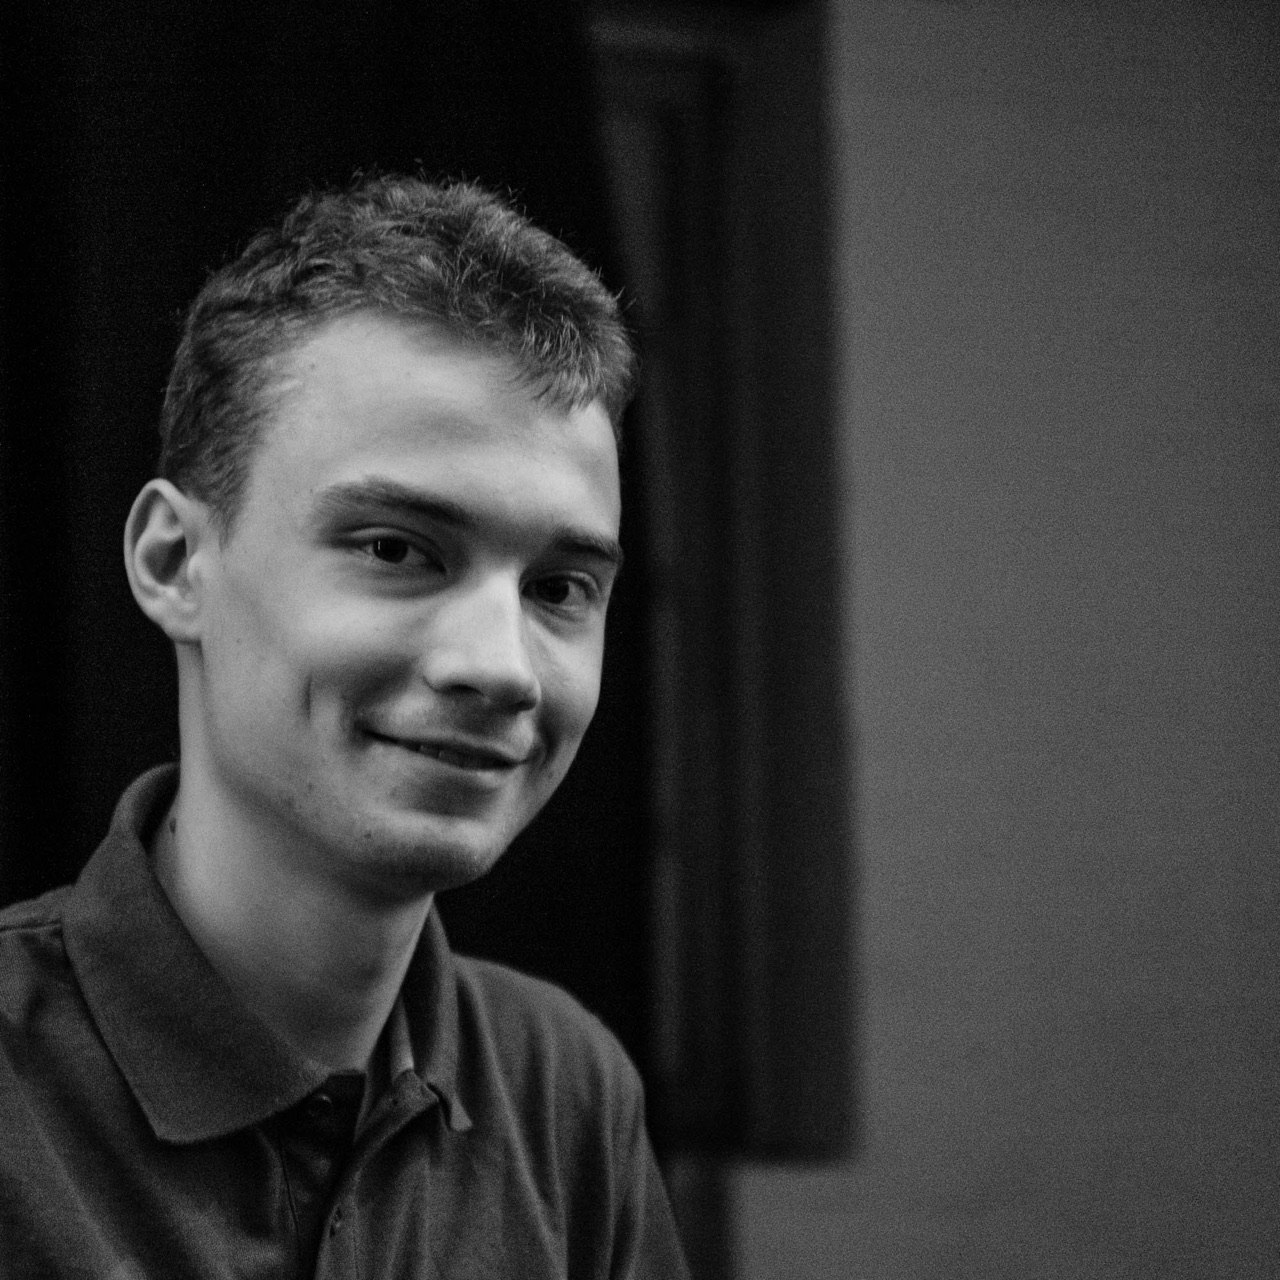
\includegraphics[width=0.4\textwidth]{Gosha.jpg}
    %\label{fig:my_label}
\end{figure}


Ольга Сучкова \\
suchkovaolga.91@mail.ru
\begin{figure}
    \centering
    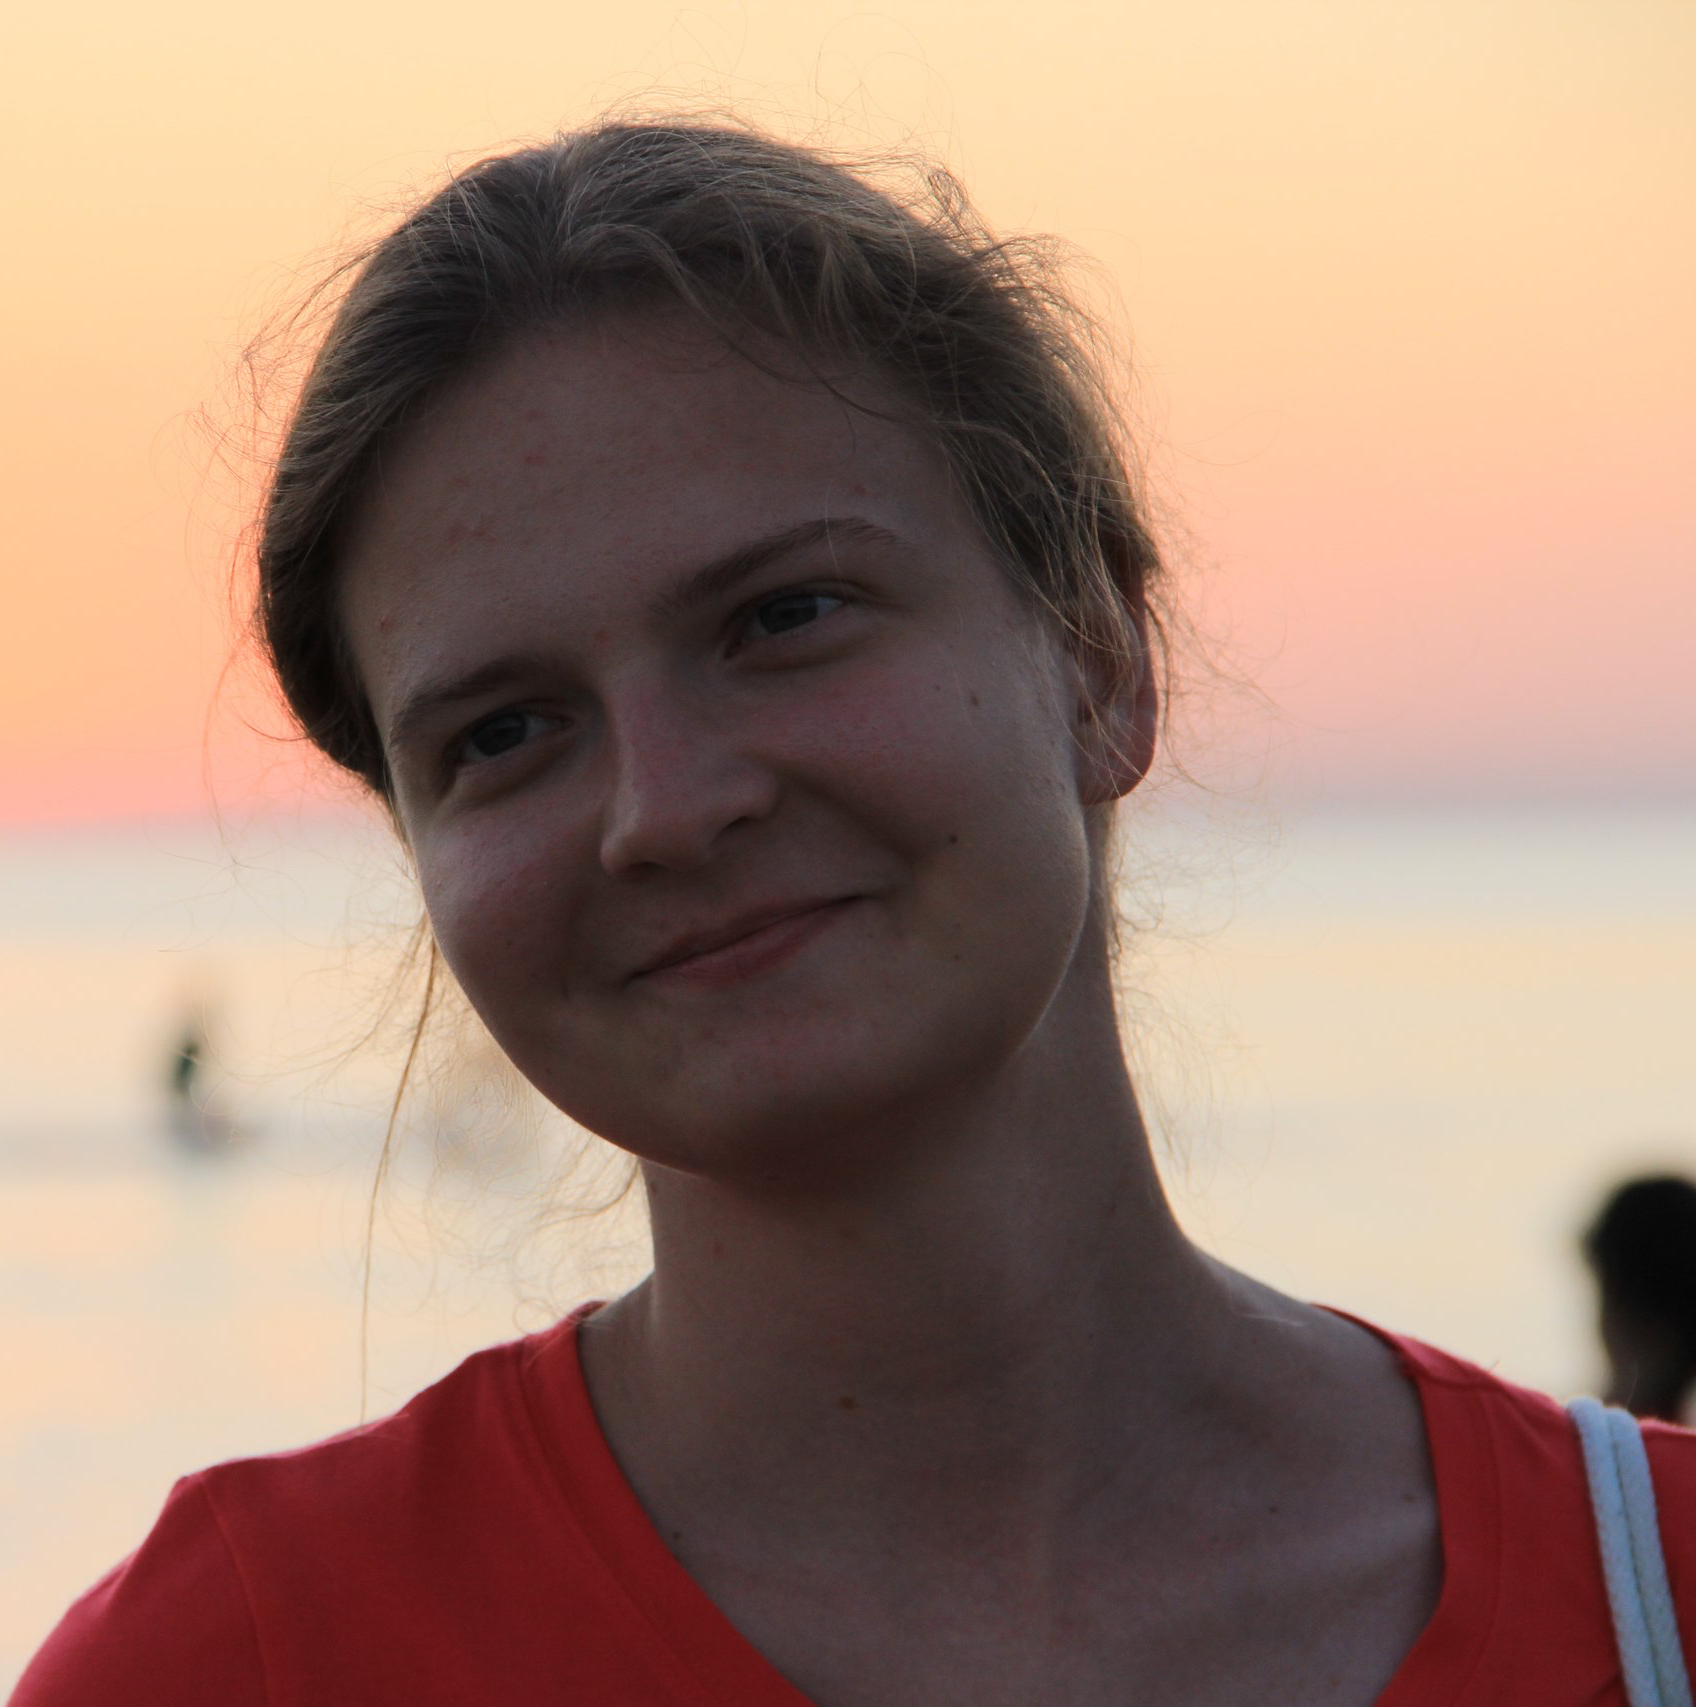
\includegraphics[width=0.4\textwidth]{Olya.jpg}
    
    %\label{fig:my_label}
\end{figure}
\end{multicols}


\end{frame}



\begin{frame}{На какие вопросы можно ответить?}

\begin{itemize}
        \item Как изменится занятость в результате
принятия закона о минимальной заработной плате?
        \item Как размер школьного класса влияет на
эффективность обучения школьников?
        \item Как изекится заболеваемость ВИЧ среди школьниц в Кении после провестительских лекций и/или раздачи бесплатных средств защиты?
\end{itemize}



\end{frame}


\begin{frame}{За <<экспериментальный подход к борьбе с глобальной бедностью>>}
% тут нужна попса про Нобелевскую премию Дюфло и Банерджи
\begin{figure}
    \centering
    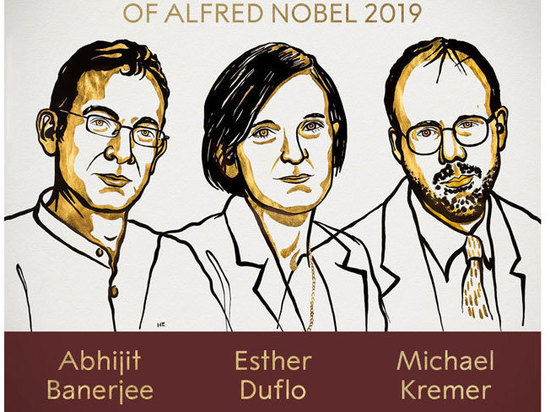
\includegraphics[width=0.8\textwidth]{Nobel 2019.jpg}
    \label{fig:my_label}
\end{figure}

\end{frame}